\section{Pre-processing and Data Modelling}
Common for many of the algorithms for finding user mobility features is that they rely on some sort of clustering of data points, to reduce the initial amount of data points into clusters representing locations where the participant did not move around a lot. For spatial clustering such as 2D data points on the surface of the earth, many of the algorithms use the DBSCAN algorithm proposed in 1996  \cite{density-based-1996} which uses the density of data points to cluster them rather than a pure distance metric such as with the K-Means algorithm. \\

In \cite{sparse-location-2014} a basic modelling approach for pre-processing is provided, which will be used for this thesis. The pre-processing produces intermediate features from which the final mobility features are derived. \\

In order to extract relevant mobility patterns, we define a few useful concepts that can be extracted from sequences of location samples. The methods described in this section are inspired by the techniques introduced in [Cuttone et al. 2014] and [Canzian et al. 2015]. We define places as specific locations of relevance to the user, such as home or workplace. Then stops are specific visits to any of those places. Thus, a stop is always associated with a single place while places can be associated with one or more stops. Finally, moves are the sequences of location samples in between stops, representing moving between places. Stops, places and moves are extracted from sequences of location samples by applying the following algorithm. To identify stops, location samples are traversed sequentially and grouped according to a maximum distance threshold. If a sample is too far from the current group median location, a new group is formed. Initially this strategy creates a lot of groups, which are then filtered by a minimum duration threshold leaving groups where movement stopped for at least some time. Each remaining group represents a stop, described by the median coordinates of the group of location samples and arrival and departure time based on the first and last location sample in the group. The appropriate values of maximum distance and minimum duration depends on the accuracy and sample frequency of the data. We applied a minimum distance of 50 meters and minimum duration of 20 minutes based on inspecting the distributions of distances and times between subsequent location samples in the dataset.

As an intermediate step, stops that are close in terms of time and distance and have no other stops in between are merged to reduce noise caused by outlier location samples that might break a stop into several stops. We merged stops that were maximum 5 minutes and 5 meters apart and found that this removed cases with a suspicious amount of stops per day. With the stops available, places are identified by clustering stops using the DBSCAN clustering algorithm [Ester et al. 1996] with a minimum cluster size of 1, effectively identifying stops appearing at the same location. Each place is represented by the median coordinates of the included stops along with a unique place ID. The place ID is also appended to each of the included stops associating each stop with a place. We applied a maximum distance of 50 meters between stops when computing the clusters.

Moves where identified by selecting the sequences of location samples in between stops. Each move is described by departure and arrival time based on the first and last location sample in the sequence, the origin and destination place ID and the total distance between the location samples in the sequence. The moves were filtered by a minimum duration and minimum distance. We applied a minimum duration of 5 minutes and a minimum distance of 50 meters. Daily features derived from the stops, places and moves include stops count, stops total duration, places count, moves count, moves total distance and moves total duration.

\textbf{Location:} $l = (lat, lon)$ \\ 
A location is defined by a geographical latitude and longitude. \\

\textbf{Single Location Data Point:} $d = (l, t)$\\
A single location data point $d$ containing a location as well as a timestamp. Some APIs may also provide the speed of the user as well as the accuracy of the data-point, but this will not be relied upon.\\

\textbf{Stop:} $s = (D, id)$\\
A stop is a visit at a known place for an extended period of time. A stop is defined by a set of single location data points $D$ as well as a \verb|Place| identifier, which if not specified will be -1, indicating that it does not belong to a \verb|Place| and is classified as noise. From the location data, an arrival-time $t_a$ and departure-time $t_d$ can be derived, as well as the duration of time spent at the stop can be derived, i.e. the difference between departure and arrival.\\

\textbf{Place:} $p = (id, S)$\\
Also referred to as a \textit{Place of Interest}, is a cluster of \verb|Stops| found by the DBSCAN algorithm \cite{density-based-1996}, which is also where the identifier $id$ comes from. When a place is generated, each stop $s \in S$ will be assigned the same identifier as the current place.\\

\textbf{Move:} $m = (s_a, s_b, D)$\\
A move is the displacement of the user from stop $s_a$ to stop $s_b$ in which the user passes through the points contained in the 'chain' of points $D$. Additional features such as the \textit{duration} of the move, the \textit{distance} between all the points (length of the point chain), and therefore also the mean transportation \textit{speed} between the two places can be derived.\\
An extensive amount of implementation of this has been done by Jonas Busk for performing this pre-processing the raw GPS data. This implementation has been carried out in Python and processes data in the offline-fashion. A large amount of this implementation will be used and referenced since it is possible to implement this in other programming languages such as Dart, which will be the main programming language of this thesis.

\subsection{Object-oriented Modelling}
In order to capture this data model with the above definitions in an object-oriented programming language such as Dart, a UML diagram was created along with the implementation to keep track of relationships between the classes. As a general rule of thumb, all the fields were made public including those required by the constructors, and the methods of the classes were all \textit{getters}, i.e. 

\begin{figure}
    \centering
    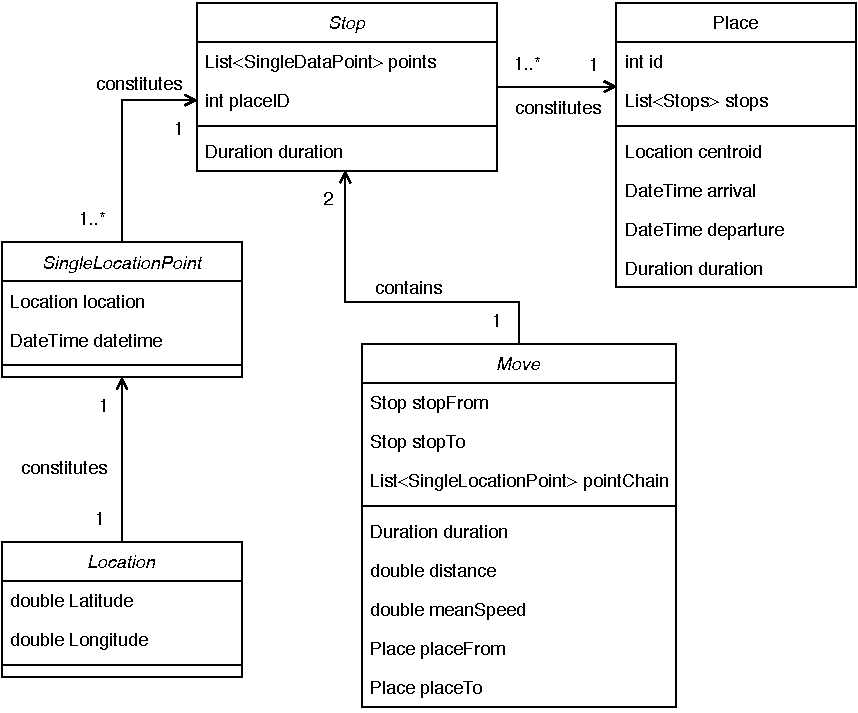
\includegraphics[width=\textwidth]{./images/Mobility-Preprocessing.pdf}
    \caption{UML diagram for the classes used for pre-processing the location data. All fields shown are public and all methods represent the derived pre-processing features}
    \label{fig:my_label}
\end{figure}
